\section{Resoconto attività di verifica}
\subsection{Periodo di analisi}
In questo paragrafo vengono analizzate le metriche \textit{MPC01, MPC02, MPC03, MPC04, MPC05, MPD01}, i restanti verranno analizzati nella successiva fase di progettazione e codifica.
\subsubsection{MPC01}
Rappresenta il valore delle attività realizzate alla data corrente.
Sull'asse delle ascisse troviamo l'unità di tempo in settimane, mentre in quello delle ordinate il valore in euro.
\begin{figure}[H]
\centering
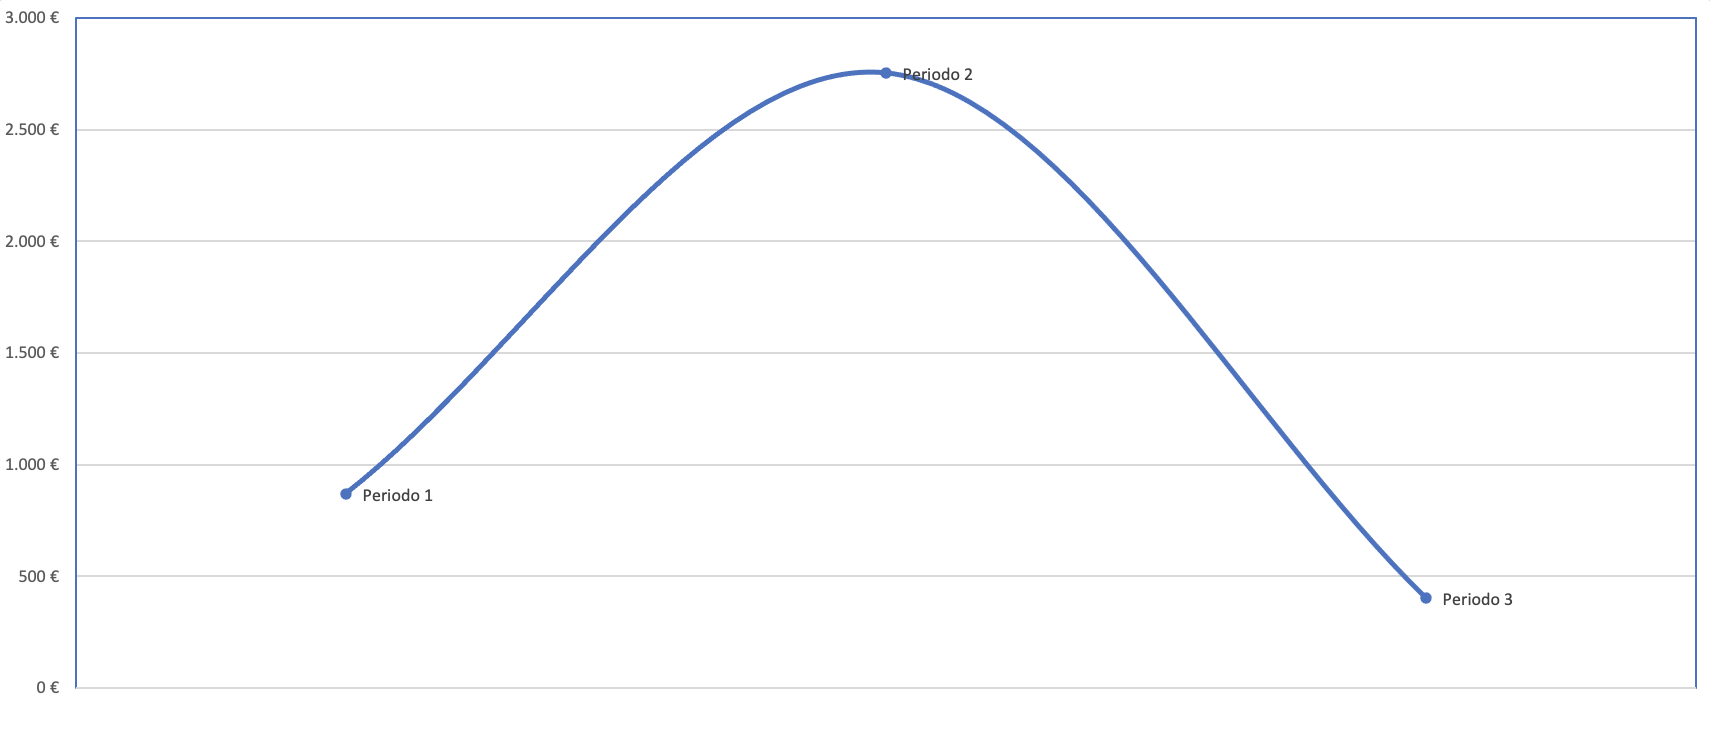
\includegraphics[width=1\textwidth]{src/img/grafico_EV.png}
\caption{Grafico EV}
\end{figure}

\subsubsection{MPC02}
Rappresenta il costo effettivamente sostenuto alla data corrente.
Sull'asse delle ascisse troviamo l'unità di tempo in settimane, mentre in quello delle ordinate il valore in euro.
\begin{figure}[H]
\centering
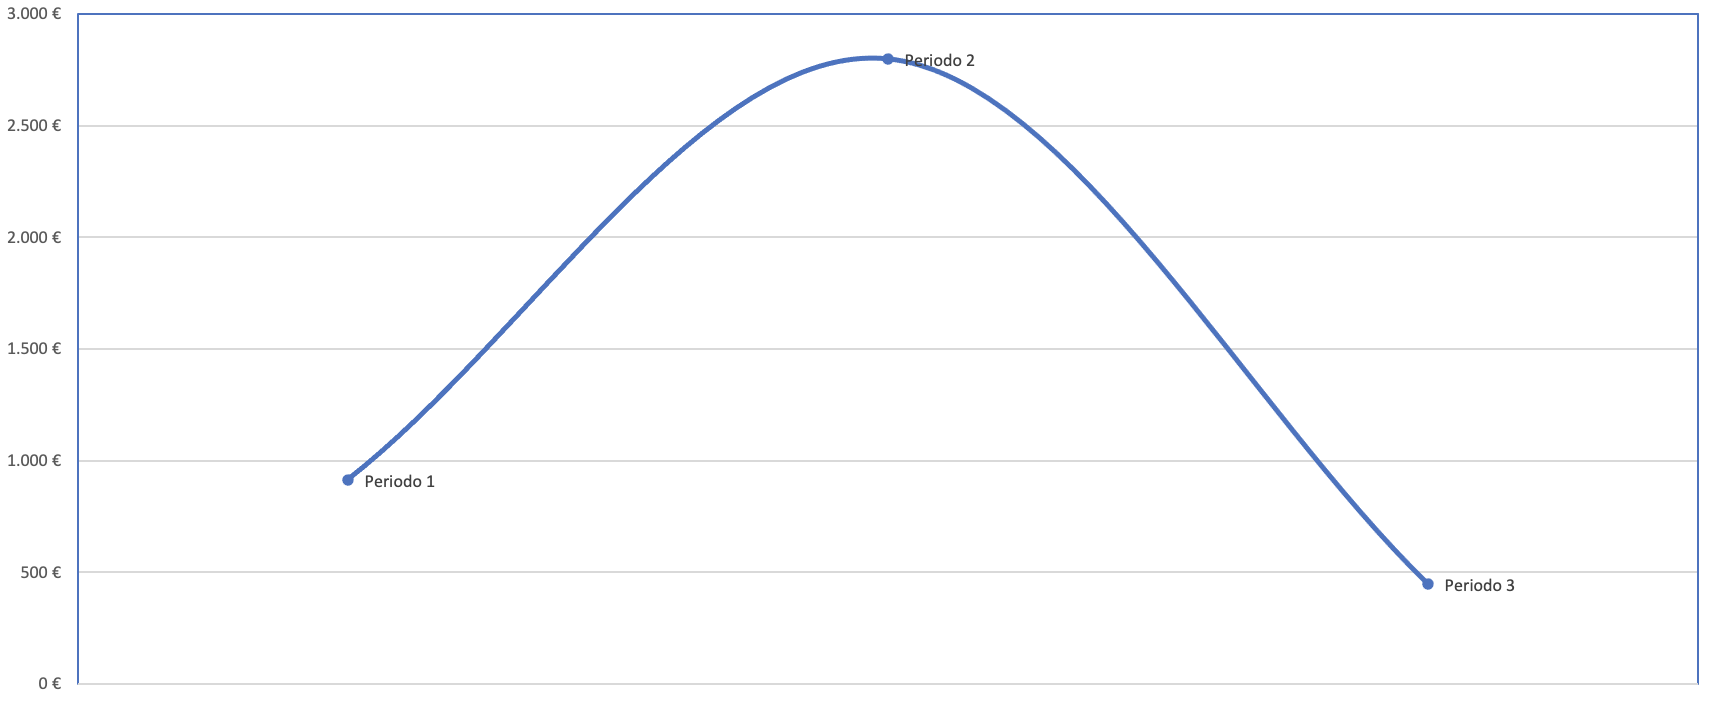
\includegraphics[width=1\textwidth]{src/img/grafico_AC.png}
\caption{Grafico AC}
\end{figure}

\subsubsection{MPC03}
Rappresenta il costo pianificato per realizzare le attività di progetto alla data corrente.
Sull'asse delle ascisse troviamo l'unità di tempo in settimane, mentre in quello delle ordinate il valore in euro.
\begin{figure}[H]
\centering
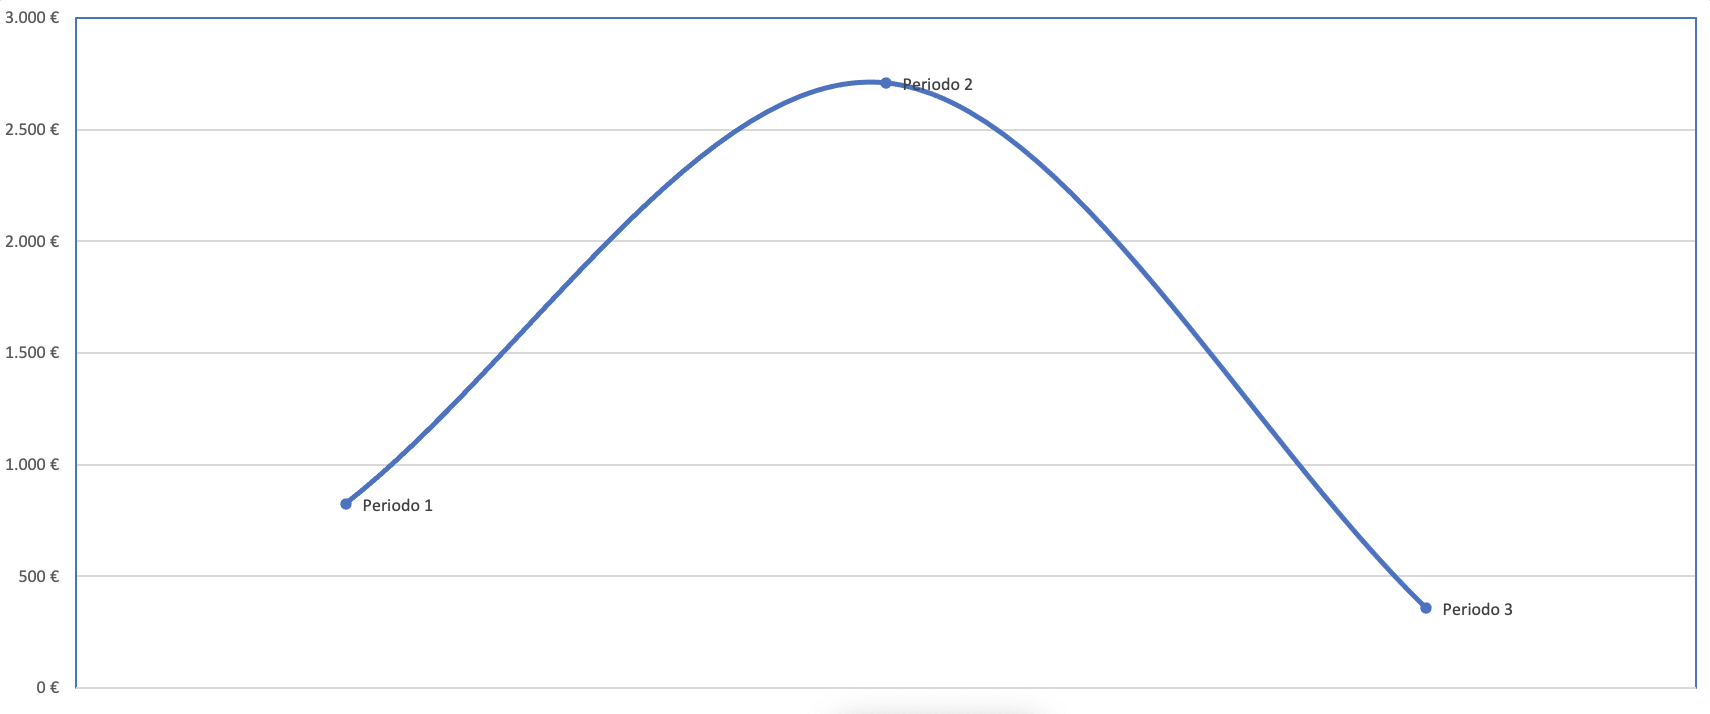
\includegraphics[width=1\textwidth]{src/img/grafico_PV.png}
\caption{Grafico PV}
\end{figure}

\subsubsection{MPC04}
Indica se il valore del costo realmente maturato è maggiore, uguale o minore rispetto al costo effettivo.
Sull'asse delle ascisse troviamo l'unità di tempo in settimane, mentre in quello delle ordinate la variazione in percentuale.
\begin{figure}[H]
\centering
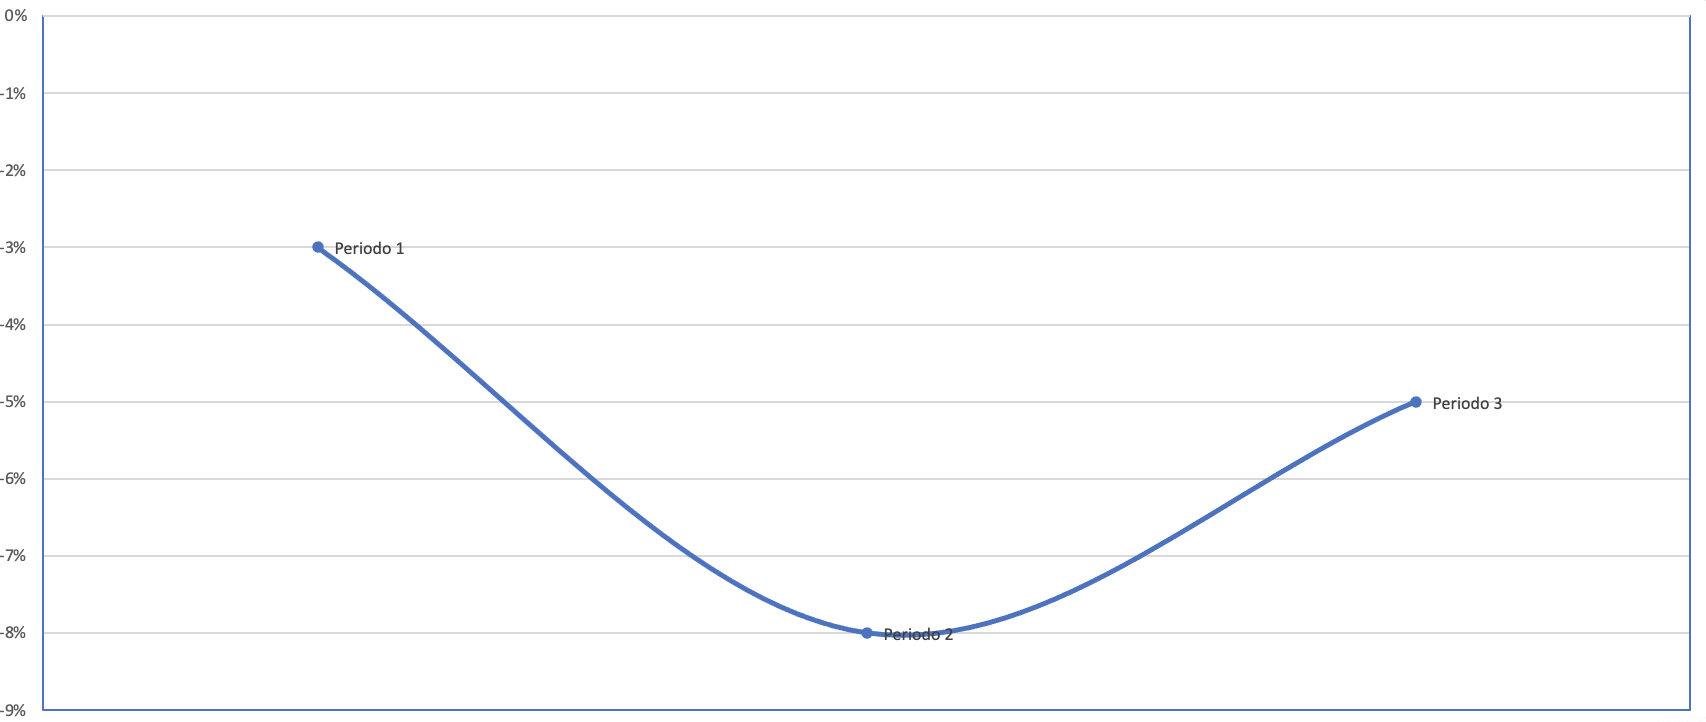
\includegraphics[width=1\textwidth]{src/img/grafico_CV.png}
\caption{Grafico CV}
\end{figure}

\subsubsection{MPC05}
Indica se si è in linea, in anticipo o in ritardo rispetto alla schedulazione delle attività di progetto pianificate nella baseline.
Sull'asse delle ascisse troviamo l'unità di tempo in settimane, mentre in quello delle ordinate la variazione in percentuale.
\begin{figure}[H]
\centering
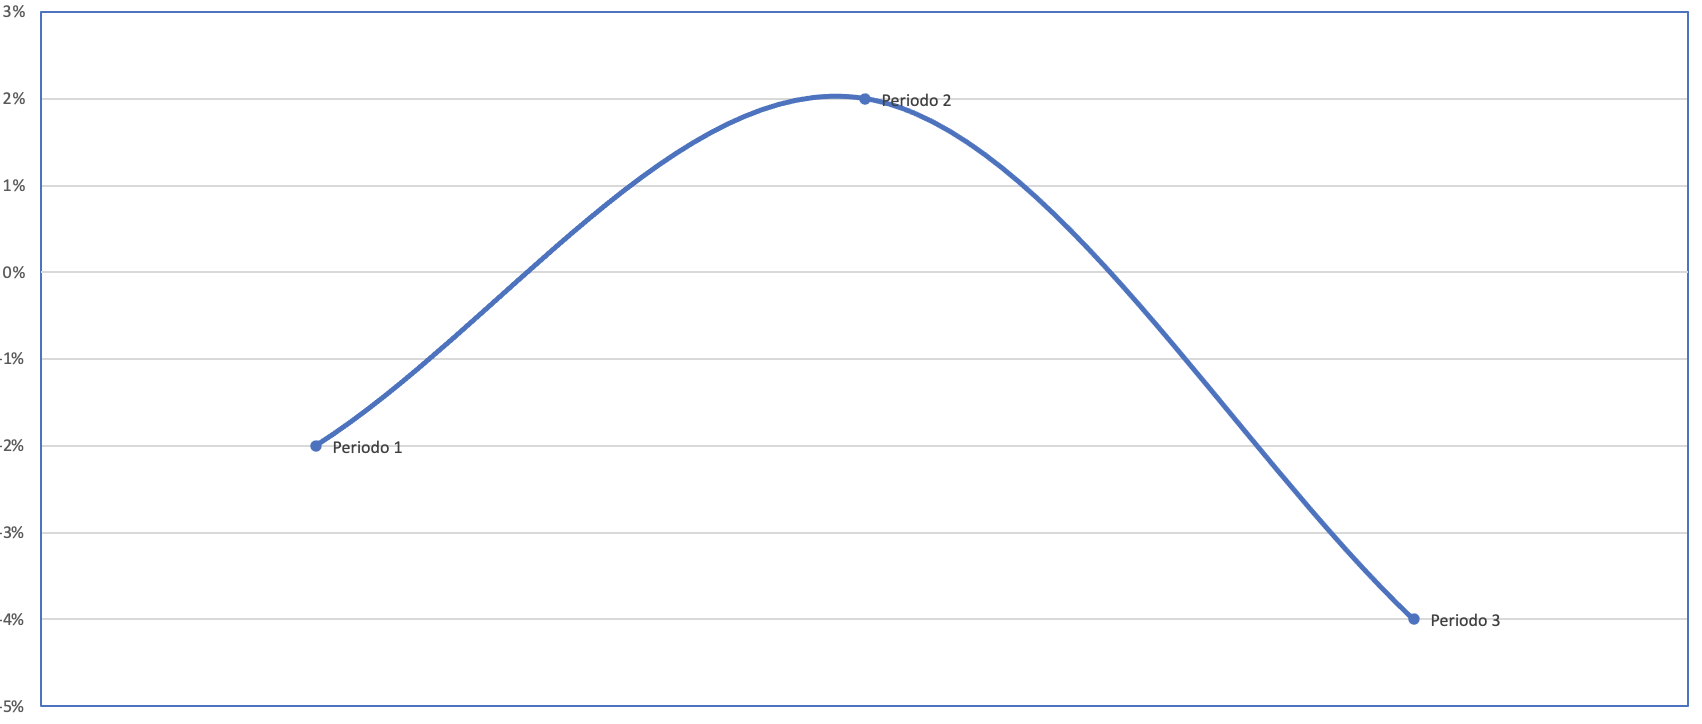
\includegraphics[width=1\textwidth]{src/img/grafico_SV.png}
\caption{Grafico SV}
\end{figure}

\subsubsection{MPD01}
L'Indice Gulpease è un indice di leggibilità di un testo tarato sulla lingua italiana. Rispetto ad altri ha il vantaggio di utilizzare la lunghezza delle parole in lettere anziché in sillabe, semplificandone il calcolo automatico.
I risultati sono compresi tra 0 e 100, dove il valore "100" indica la leggibilità più alta e "0" la leggibilità più bassa. In generale risulta che testi con un indice
\begin{itemize}
    \item inferiore a 80 sono difficili da leggere per chi ha la licenza elementare;
    \item inferiore a 60 sono difficili da leggere per chi ha la licenza media;
    \item inferiore a 40 sono difficili da leggere per chi ha un diploma superiore.
\end{itemize}

Di seguito vengono mostrati i risultati dell’indice di Gulpease per ogni documento redatto, escludendone la prima pagina, registro delle modifiche, l'indice e gli elenchi di figure e tabelle.

\renewcommand{\arraystretch}{1.8}
\begin{xltabular}{\textwidth} {
        >{\hsize=1.4\hsize\linewidth=\hsize}X
        >{\hsize=0.8\hsize\linewidth=\hsize}X
        >{\hsize=1\hsize\linewidth=\hsize}X
    }
    \rowcolorhead
    \textbf{\color{white}Documento} &
    \textbf{\color{white}Valore indice} &
    \textbf{\color{white}Esito}\\
    \hline
    \endfirsthead

    \hline
    \rowcolorhead
    \textbf{\color{white}Documento} &
    \textbf{\color{white}Valore indice} &
    \textbf{\color{white}Esito}\\
    \hline
    \endhead

    \endfoot

    \endlastfoot

    \textit{Analisi dei Requisiti v1.0.0}&
    68 &
    Superato
    \\ \hline

    \textit{Norme di Progetto v1.0.0}&
    68 &
    Superato
    \\ \hline

    \textit{Piano di Progetto v1.0.0}&
    68 &
    Superato
    \\ \hline

    \textit{Piano di Qualifica v1.0.0}&
    68 &
    Superato
    \\ \hline

    \textit{Glossario v1.0.0}&
    68 &
    Superato
    \\ \hline

    \textit{Verbali}&
    68 &
    Superato
    \\ \hline


    \rowcolor{white}
    \caption{Risultati indice di Gulpease}
\end{xltabular}










